% Created by tikzDevice version 0.11 on 2018-08-15 18:27:50
% !TEX encoding = UTF-8 Unicode
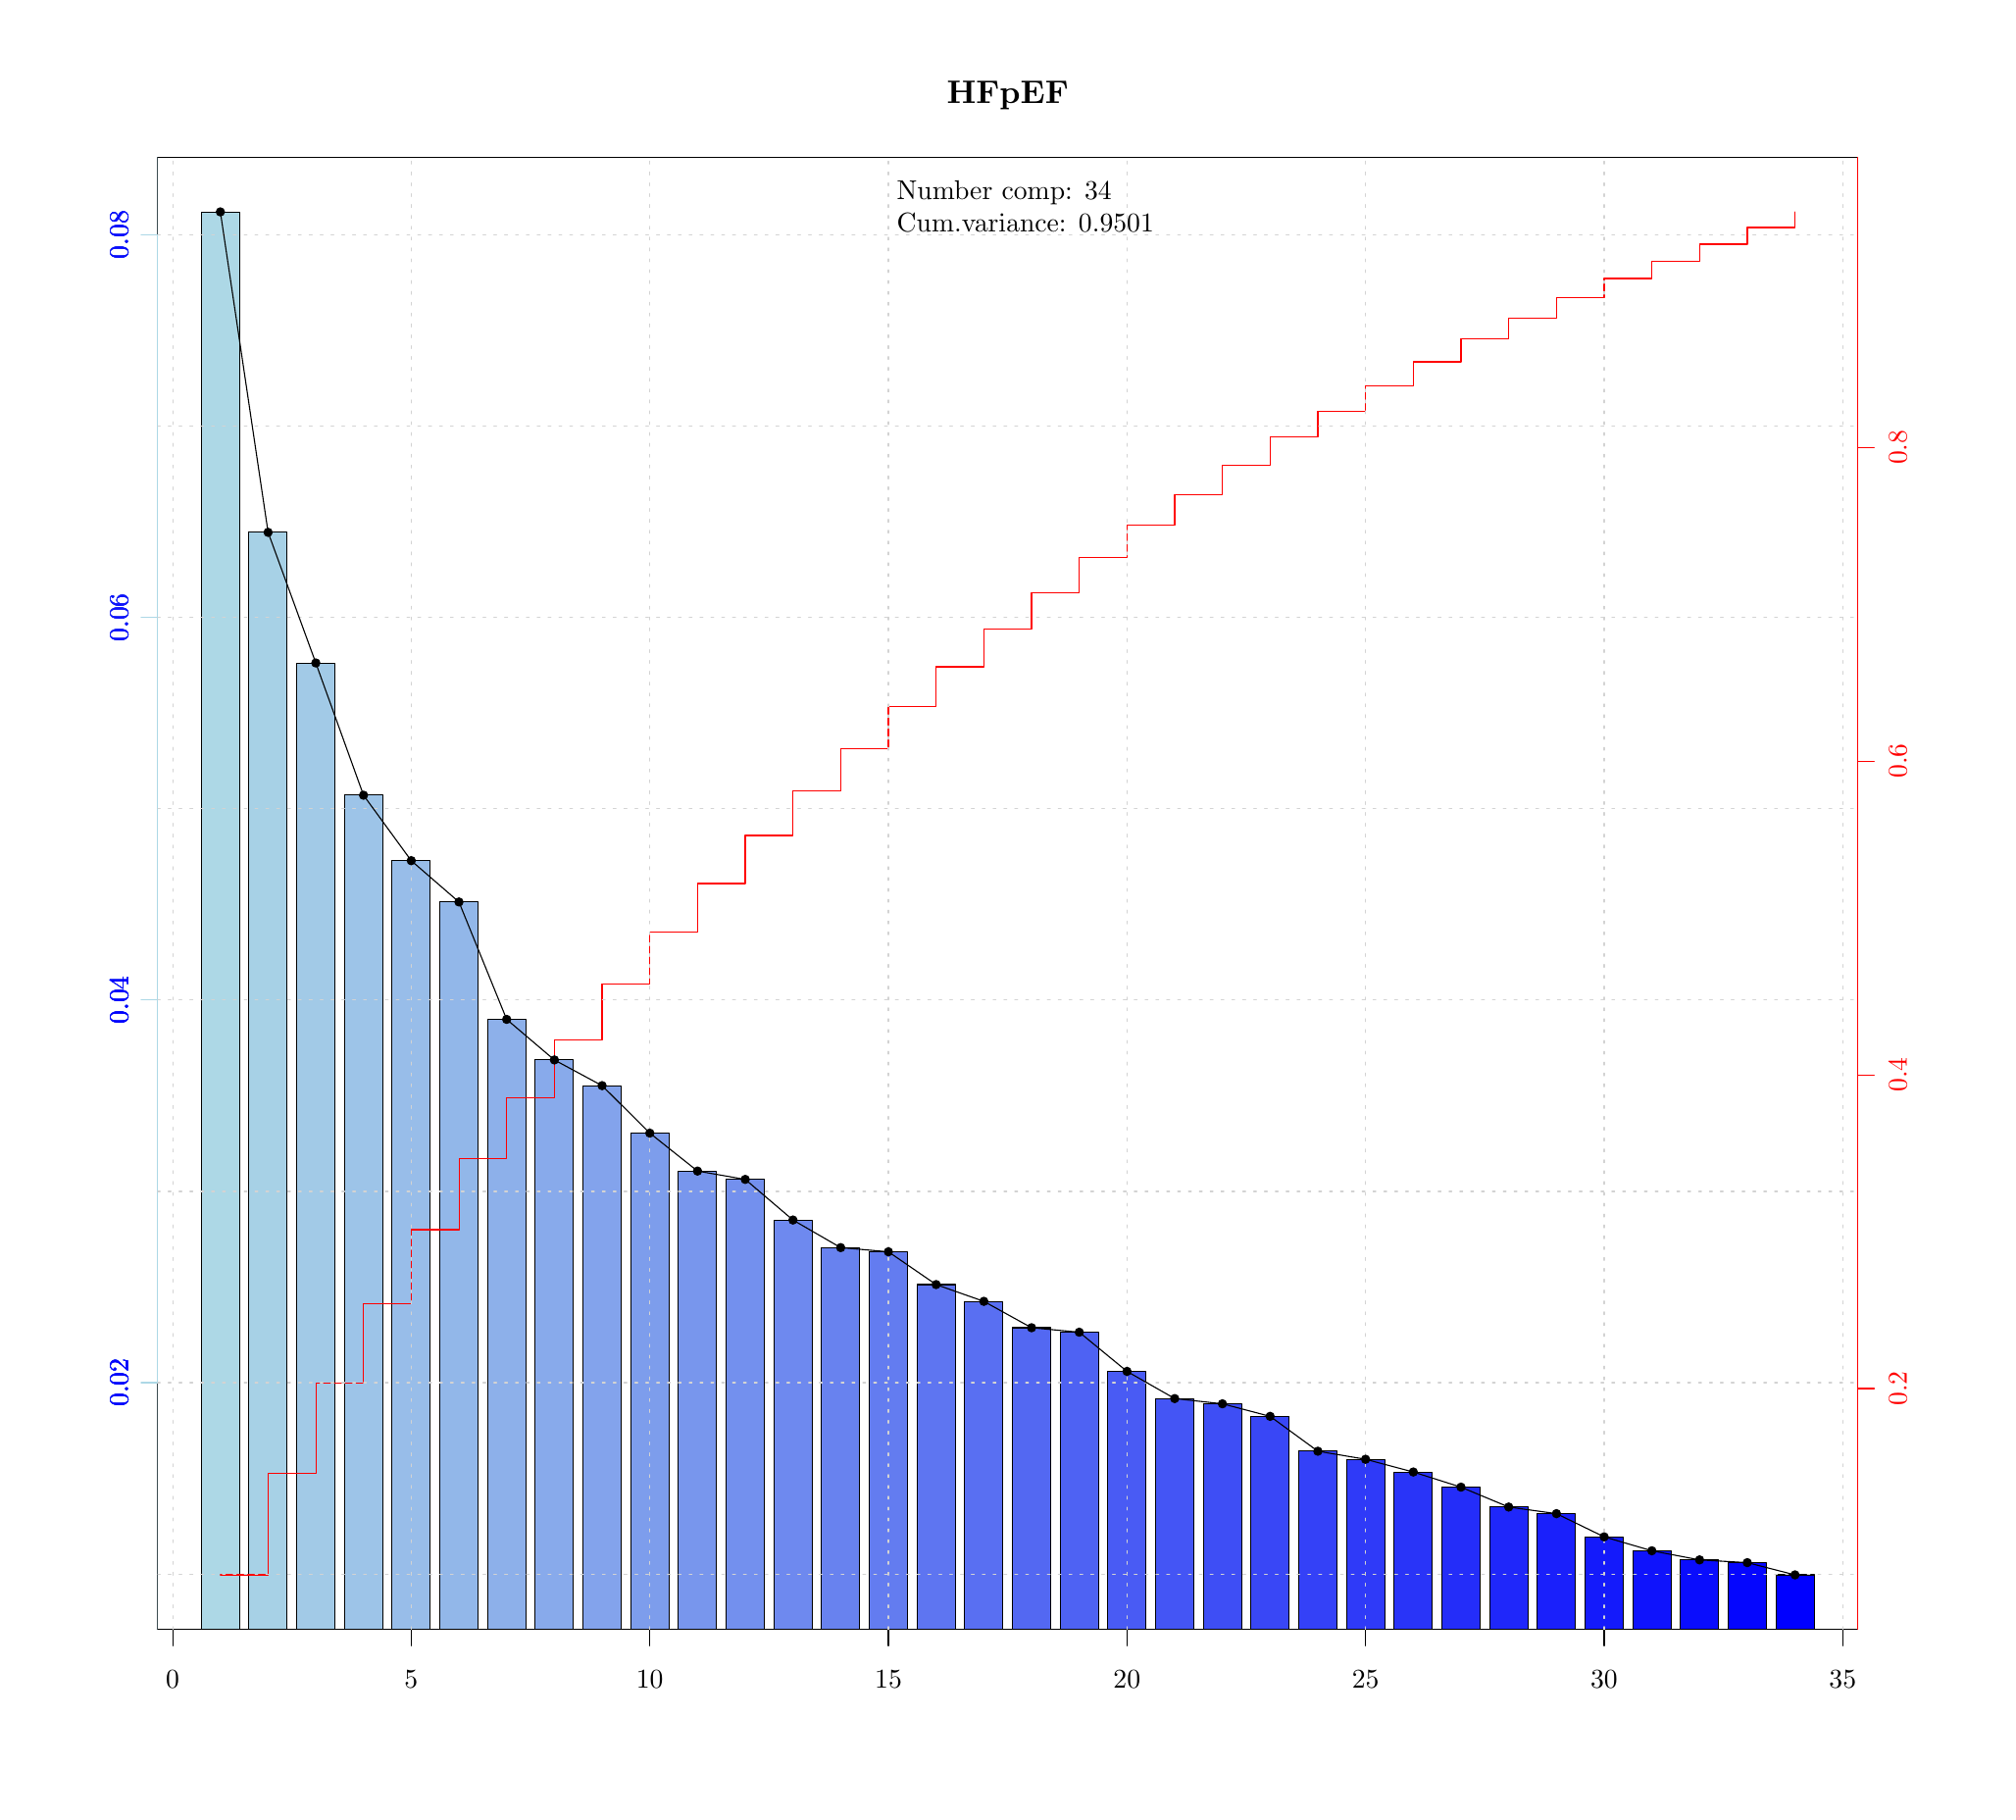
\begin{tikzpicture}[x=1pt,y=1pt]
\definecolor{fillColor}{RGB}{255,255,255}
\path[use as bounding box,fill=fillColor,fill opacity=0.00] (0,0) rectangle (722.70,650.43);
\begin{scope}
\path[clip] ( 48.00, 60.00) rectangle (674.70,602.43);
\definecolor{drawColor}{RGB}{0,0,0}
\definecolor{fillColor}{RGB}{173,216,230}

\path[draw=drawColor,line width= 0.4pt,line join=round,line cap=round,fill=fillColor] ( 64.18, 60.00) rectangle ( 78.24,582.34);
\definecolor{fillColor}{RGB}{167,209,230}

\path[draw=drawColor,line width= 0.4pt,line join=round,line cap=round,fill=fillColor] ( 81.76, 60.00) rectangle ( 95.83,464.25);
\definecolor{fillColor}{RGB}{162,202,231}

\path[draw=drawColor,line width= 0.4pt,line join=round,line cap=round,fill=fillColor] ( 99.35, 60.00) rectangle (113.41,416.12);
\definecolor{fillColor}{RGB}{157,196,232}

\path[draw=drawColor,line width= 0.4pt,line join=round,line cap=round,fill=fillColor] (116.93, 60.00) rectangle (131.00,367.39);
\definecolor{fillColor}{RGB}{152,189,233}

\path[draw=drawColor,line width= 0.4pt,line join=round,line cap=round,fill=fillColor] (134.51, 60.00) rectangle (148.58,343.27);
\definecolor{fillColor}{RGB}{146,183,233}

\path[draw=drawColor,line width= 0.4pt,line join=round,line cap=round,fill=fillColor] (152.10, 60.00) rectangle (166.17,328.05);
\definecolor{fillColor}{RGB}{141,176,234}

\path[draw=drawColor,line width= 0.4pt,line join=round,line cap=round,fill=fillColor] (169.68, 60.00) rectangle (183.75,284.78);
\definecolor{fillColor}{RGB}{136,170,235}

\path[draw=drawColor,line width= 0.4pt,line join=round,line cap=round,fill=fillColor] (187.27, 60.00) rectangle (201.33,269.84);
\definecolor{fillColor}{RGB}{131,163,236}

\path[draw=drawColor,line width= 0.4pt,line join=round,line cap=round,fill=fillColor] (204.85, 60.00) rectangle (218.92,260.37);
\definecolor{fillColor}{RGB}{125,157,236}

\path[draw=drawColor,line width= 0.4pt,line join=round,line cap=round,fill=fillColor] (222.44, 60.00) rectangle (236.50,242.88);
\definecolor{fillColor}{RGB}{120,150,237}

\path[draw=drawColor,line width= 0.4pt,line join=round,line cap=round,fill=fillColor] (240.02, 60.00) rectangle (254.09,228.89);
\definecolor{fillColor}{RGB}{115,144,238}

\path[draw=drawColor,line width= 0.4pt,line join=round,line cap=round,fill=fillColor] (257.60, 60.00) rectangle (271.67,225.82);
\definecolor{fillColor}{RGB}{110,137,239}

\path[draw=drawColor,line width= 0.4pt,line join=round,line cap=round,fill=fillColor] (275.19, 60.00) rectangle (289.25,210.85);
\definecolor{fillColor}{RGB}{104,130,239}

\path[draw=drawColor,line width= 0.4pt,line join=round,line cap=round,fill=fillColor] (292.77, 60.00) rectangle (306.84,200.68);
\definecolor{fillColor}{RGB}{99,124,240}

\path[draw=drawColor,line width= 0.4pt,line join=round,line cap=round,fill=fillColor] (310.36, 60.00) rectangle (324.42,199.15);
\definecolor{fillColor}{RGB}{94,117,241}

\path[draw=drawColor,line width= 0.4pt,line join=round,line cap=round,fill=fillColor] (327.94, 60.00) rectangle (342.01,187.07);
\definecolor{fillColor}{RGB}{89,111,242}

\path[draw=drawColor,line width= 0.4pt,line join=round,line cap=round,fill=fillColor] (345.52, 60.00) rectangle (359.59,180.88);
\definecolor{fillColor}{RGB}{83,104,242}

\path[draw=drawColor,line width= 0.4pt,line join=round,line cap=round,fill=fillColor] (363.11, 60.00) rectangle (377.18,171.16);
\definecolor{fillColor}{RGB}{78,98,243}

\path[draw=drawColor,line width= 0.4pt,line join=round,line cap=round,fill=fillColor] (380.69, 60.00) rectangle (394.76,169.51);
\definecolor{fillColor}{RGB}{73,91,244}

\path[draw=drawColor,line width= 0.4pt,line join=round,line cap=round,fill=fillColor] (398.28, 60.00) rectangle (412.34,155.08);
\definecolor{fillColor}{RGB}{68,85,245}

\path[draw=drawColor,line width= 0.4pt,line join=round,line cap=round,fill=fillColor] (415.86, 60.00) rectangle (429.93,145.06);
\definecolor{fillColor}{RGB}{62,78,245}

\path[draw=drawColor,line width= 0.4pt,line join=round,line cap=round,fill=fillColor] (433.45, 60.00) rectangle (447.51,143.13);
\definecolor{fillColor}{RGB}{57,71,246}

\path[draw=drawColor,line width= 0.4pt,line join=round,line cap=round,fill=fillColor] (451.03, 60.00) rectangle (465.10,138.51);
\definecolor{fillColor}{RGB}{52,65,247}

\path[draw=drawColor,line width= 0.4pt,line join=round,line cap=round,fill=fillColor] (468.61, 60.00) rectangle (482.68,125.66);
\definecolor{fillColor}{RGB}{47,58,248}

\path[draw=drawColor,line width= 0.4pt,line join=round,line cap=round,fill=fillColor] (486.20, 60.00) rectangle (500.26,122.69);
\definecolor{fillColor}{RGB}{41,52,248}

\path[draw=drawColor,line width= 0.4pt,line join=round,line cap=round,fill=fillColor] (503.78, 60.00) rectangle (517.85,118.00);
\definecolor{fillColor}{RGB}{36,45,249}

\path[draw=drawColor,line width= 0.4pt,line join=round,line cap=round,fill=fillColor] (521.37, 60.00) rectangle (535.43,112.42);
\definecolor{fillColor}{RGB}{31,39,250}

\path[draw=drawColor,line width= 0.4pt,line join=round,line cap=round,fill=fillColor] (538.95, 60.00) rectangle (553.02,105.09);
\definecolor{fillColor}{RGB}{26,32,251}

\path[draw=drawColor,line width= 0.4pt,line join=round,line cap=round,fill=fillColor] (556.53, 60.00) rectangle (570.60,102.65);
\definecolor{fillColor}{RGB}{20,26,251}

\path[draw=drawColor,line width= 0.4pt,line join=round,line cap=round,fill=fillColor] (574.12, 60.00) rectangle (588.19, 94.11);
\definecolor{fillColor}{RGB}{15,19,252}

\path[draw=drawColor,line width= 0.4pt,line join=round,line cap=round,fill=fillColor] (591.70, 60.00) rectangle (605.77, 88.97);
\definecolor{fillColor}{RGB}{10,13,253}

\path[draw=drawColor,line width= 0.4pt,line join=round,line cap=round,fill=fillColor] (609.29, 60.00) rectangle (623.35, 85.61);
\definecolor{fillColor}{RGB}{5,6,254}

\path[draw=drawColor,line width= 0.4pt,line join=round,line cap=round,fill=fillColor] (626.87, 60.00) rectangle (640.94, 84.60);
\definecolor{fillColor}{RGB}{0,0,255}

\path[draw=drawColor,line width= 0.4pt,line join=round,line cap=round,fill=fillColor] (644.46, 60.00) rectangle (658.52, 80.09);
\end{scope}
\begin{scope}
\path[clip] (  0.00,  0.00) rectangle (722.70,650.43);
\definecolor{drawColor}{RGB}{0,0,0}

\node[text=drawColor,anchor=base,inner sep=0pt, outer sep=0pt, scale=  1.20] at (361.35,622.29) {\bfseries HFpEF};
\end{scope}
\begin{scope}
\path[clip] (  0.00,  0.00) rectangle (722.70,650.43);
\definecolor{drawColor}{RGB}{0,0,0}

\path[draw=drawColor,line width= 0.4pt,line join=round,line cap=round] ( 48.00, 60.00) --
	(674.70, 60.00) --
	(674.70,602.43) --
	( 48.00,602.43) --
	( 48.00, 60.00);

\path[draw=drawColor,line width= 0.4pt,line join=round,line cap=round] ( 53.63, 60.00) -- (669.07, 60.00);

\path[draw=drawColor,line width= 0.4pt,line join=round,line cap=round] ( 53.63, 60.00) -- ( 53.63, 54.00);

\path[draw=drawColor,line width= 0.4pt,line join=round,line cap=round] (141.55, 60.00) -- (141.55, 54.00);

\path[draw=drawColor,line width= 0.4pt,line join=round,line cap=round] (229.47, 60.00) -- (229.47, 54.00);

\path[draw=drawColor,line width= 0.4pt,line join=round,line cap=round] (317.39, 60.00) -- (317.39, 54.00);

\path[draw=drawColor,line width= 0.4pt,line join=round,line cap=round] (405.31, 60.00) -- (405.31, 54.00);

\path[draw=drawColor,line width= 0.4pt,line join=round,line cap=round] (493.23, 60.00) -- (493.23, 54.00);

\path[draw=drawColor,line width= 0.4pt,line join=round,line cap=round] (581.15, 60.00) -- (581.15, 54.00);

\path[draw=drawColor,line width= 0.4pt,line join=round,line cap=round] (669.07, 60.00) -- (669.07, 54.00);

\node[text=drawColor,anchor=base,inner sep=0pt, outer sep=0pt, scale=  1.00] at ( 53.63, 38.40) {0};

\node[text=drawColor,anchor=base,inner sep=0pt, outer sep=0pt, scale=  1.00] at (141.55, 38.40) {5};

\node[text=drawColor,anchor=base,inner sep=0pt, outer sep=0pt, scale=  1.00] at (229.47, 38.40) {10};

\node[text=drawColor,anchor=base,inner sep=0pt, outer sep=0pt, scale=  1.00] at (317.39, 38.40) {15};

\node[text=drawColor,anchor=base,inner sep=0pt, outer sep=0pt, scale=  1.00] at (405.31, 38.40) {20};

\node[text=drawColor,anchor=base,inner sep=0pt, outer sep=0pt, scale=  1.00] at (493.23, 38.40) {25};

\node[text=drawColor,anchor=base,inner sep=0pt, outer sep=0pt, scale=  1.00] at (581.15, 38.40) {30};

\node[text=drawColor,anchor=base,inner sep=0pt, outer sep=0pt, scale=  1.00] at (669.07, 38.40) {35};
\definecolor{drawColor}{RGB}{173,216,230}

\path[draw=drawColor,line width= 0.4pt,line join=round,line cap=round] ( 48.00,150.91) -- ( 48.00,573.84);

\path[draw=drawColor,line width= 0.4pt,line join=round,line cap=round] ( 48.00,150.91) -- ( 42.00,150.91);

\path[draw=drawColor,line width= 0.4pt,line join=round,line cap=round] ( 48.00,291.89) -- ( 42.00,291.89);

\path[draw=drawColor,line width= 0.4pt,line join=round,line cap=round] ( 48.00,432.86) -- ( 42.00,432.86);

\path[draw=drawColor,line width= 0.4pt,line join=round,line cap=round] ( 48.00,573.84) -- ( 42.00,573.84);

\node[text=drawColor,rotate= 90.00,anchor=base,inner sep=0pt, outer sep=0pt, scale=  1.00] at ( 37.20,150.91) {0.02};
\definecolor{drawColor}{RGB}{167,209,230}

\node[text=drawColor,rotate= 90.00,anchor=base,inner sep=0pt, outer sep=0pt, scale=  1.00] at ( 37.20,291.89) {0.04};
\definecolor{drawColor}{RGB}{162,202,231}

\node[text=drawColor,rotate= 90.00,anchor=base,inner sep=0pt, outer sep=0pt, scale=  1.00] at ( 37.20,432.86) {0.06};
\definecolor{drawColor}{RGB}{157,196,232}

\node[text=drawColor,rotate= 90.00,anchor=base,inner sep=0pt, outer sep=0pt, scale=  1.00] at ( 37.20,573.84) {0.08};
\definecolor{drawColor}{RGB}{152,189,233}

\node[text=drawColor,rotate= 90.00,anchor=base,inner sep=0pt, outer sep=0pt, scale=  1.00] at ( 37.20,150.91) {0.02};
\definecolor{drawColor}{RGB}{146,183,233}

\node[text=drawColor,rotate= 90.00,anchor=base,inner sep=0pt, outer sep=0pt, scale=  1.00] at ( 37.20,291.89) {0.04};
\definecolor{drawColor}{RGB}{141,176,234}

\node[text=drawColor,rotate= 90.00,anchor=base,inner sep=0pt, outer sep=0pt, scale=  1.00] at ( 37.20,432.86) {0.06};
\definecolor{drawColor}{RGB}{136,170,235}

\node[text=drawColor,rotate= 90.00,anchor=base,inner sep=0pt, outer sep=0pt, scale=  1.00] at ( 37.20,573.84) {0.08};
\definecolor{drawColor}{RGB}{131,163,236}

\node[text=drawColor,rotate= 90.00,anchor=base,inner sep=0pt, outer sep=0pt, scale=  1.00] at ( 37.20,150.91) {0.02};
\definecolor{drawColor}{RGB}{125,157,236}

\node[text=drawColor,rotate= 90.00,anchor=base,inner sep=0pt, outer sep=0pt, scale=  1.00] at ( 37.20,291.89) {0.04};
\definecolor{drawColor}{RGB}{120,150,237}

\node[text=drawColor,rotate= 90.00,anchor=base,inner sep=0pt, outer sep=0pt, scale=  1.00] at ( 37.20,432.86) {0.06};
\definecolor{drawColor}{RGB}{115,144,238}

\node[text=drawColor,rotate= 90.00,anchor=base,inner sep=0pt, outer sep=0pt, scale=  1.00] at ( 37.20,573.84) {0.08};
\definecolor{drawColor}{RGB}{110,137,239}

\node[text=drawColor,rotate= 90.00,anchor=base,inner sep=0pt, outer sep=0pt, scale=  1.00] at ( 37.20,150.91) {0.02};
\definecolor{drawColor}{RGB}{104,130,239}

\node[text=drawColor,rotate= 90.00,anchor=base,inner sep=0pt, outer sep=0pt, scale=  1.00] at ( 37.20,291.89) {0.04};
\definecolor{drawColor}{RGB}{99,124,240}

\node[text=drawColor,rotate= 90.00,anchor=base,inner sep=0pt, outer sep=0pt, scale=  1.00] at ( 37.20,432.86) {0.06};
\definecolor{drawColor}{RGB}{94,117,241}

\node[text=drawColor,rotate= 90.00,anchor=base,inner sep=0pt, outer sep=0pt, scale=  1.00] at ( 37.20,573.84) {0.08};
\definecolor{drawColor}{RGB}{89,111,242}

\node[text=drawColor,rotate= 90.00,anchor=base,inner sep=0pt, outer sep=0pt, scale=  1.00] at ( 37.20,150.91) {0.02};
\definecolor{drawColor}{RGB}{83,104,242}

\node[text=drawColor,rotate= 90.00,anchor=base,inner sep=0pt, outer sep=0pt, scale=  1.00] at ( 37.20,291.89) {0.04};
\definecolor{drawColor}{RGB}{78,98,243}

\node[text=drawColor,rotate= 90.00,anchor=base,inner sep=0pt, outer sep=0pt, scale=  1.00] at ( 37.20,432.86) {0.06};
\definecolor{drawColor}{RGB}{73,91,244}

\node[text=drawColor,rotate= 90.00,anchor=base,inner sep=0pt, outer sep=0pt, scale=  1.00] at ( 37.20,573.84) {0.08};
\definecolor{drawColor}{RGB}{68,85,245}

\node[text=drawColor,rotate= 90.00,anchor=base,inner sep=0pt, outer sep=0pt, scale=  1.00] at ( 37.20,150.91) {0.02};
\definecolor{drawColor}{RGB}{62,78,245}

\node[text=drawColor,rotate= 90.00,anchor=base,inner sep=0pt, outer sep=0pt, scale=  1.00] at ( 37.20,291.89) {0.04};
\definecolor{drawColor}{RGB}{57,71,246}

\node[text=drawColor,rotate= 90.00,anchor=base,inner sep=0pt, outer sep=0pt, scale=  1.00] at ( 37.20,432.86) {0.06};
\definecolor{drawColor}{RGB}{52,65,247}

\node[text=drawColor,rotate= 90.00,anchor=base,inner sep=0pt, outer sep=0pt, scale=  1.00] at ( 37.20,573.84) {0.08};
\definecolor{drawColor}{RGB}{47,58,248}

\node[text=drawColor,rotate= 90.00,anchor=base,inner sep=0pt, outer sep=0pt, scale=  1.00] at ( 37.20,150.91) {0.02};
\definecolor{drawColor}{RGB}{41,52,248}

\node[text=drawColor,rotate= 90.00,anchor=base,inner sep=0pt, outer sep=0pt, scale=  1.00] at ( 37.20,291.89) {0.04};
\definecolor{drawColor}{RGB}{36,45,249}

\node[text=drawColor,rotate= 90.00,anchor=base,inner sep=0pt, outer sep=0pt, scale=  1.00] at ( 37.20,432.86) {0.06};
\definecolor{drawColor}{RGB}{31,39,250}

\node[text=drawColor,rotate= 90.00,anchor=base,inner sep=0pt, outer sep=0pt, scale=  1.00] at ( 37.20,573.84) {0.08};
\definecolor{drawColor}{RGB}{26,32,251}

\node[text=drawColor,rotate= 90.00,anchor=base,inner sep=0pt, outer sep=0pt, scale=  1.00] at ( 37.20,150.91) {0.02};
\definecolor{drawColor}{RGB}{20,26,251}

\node[text=drawColor,rotate= 90.00,anchor=base,inner sep=0pt, outer sep=0pt, scale=  1.00] at ( 37.20,291.89) {0.04};
\definecolor{drawColor}{RGB}{15,19,252}

\node[text=drawColor,rotate= 90.00,anchor=base,inner sep=0pt, outer sep=0pt, scale=  1.00] at ( 37.20,432.86) {0.06};
\definecolor{drawColor}{RGB}{10,13,253}

\node[text=drawColor,rotate= 90.00,anchor=base,inner sep=0pt, outer sep=0pt, scale=  1.00] at ( 37.20,573.84) {0.08};
\definecolor{drawColor}{RGB}{5,6,254}

\node[text=drawColor,rotate= 90.00,anchor=base,inner sep=0pt, outer sep=0pt, scale=  1.00] at ( 37.20,150.91) {0.02};
\definecolor{drawColor}{RGB}{0,0,255}

\node[text=drawColor,rotate= 90.00,anchor=base,inner sep=0pt, outer sep=0pt, scale=  1.00] at ( 37.20,291.89) {0.04};
\end{scope}
\begin{scope}
\path[clip] ( 48.00, 60.00) rectangle (674.70,602.43);
\definecolor{drawColor}{RGB}{173,216,230}

\path[draw=drawColor,line width= 0.4pt,line join=round,line cap=round] ( 48.00, 60.00) -- ( 48.00,602.43);
\definecolor{drawColor}{RGB}{255,0,0}

\path[draw=drawColor,line width= 0.4pt,line join=round,line cap=round] ( 71.21, 80.09) --
	( 88.80, 80.09) --
	( 88.80,117.35) --
	(106.38,117.35) --
	(106.38,150.65) --
	(123.96,150.65) --
	(123.96,179.97) --
	(141.55,179.97) --
	(141.55,207.30) --
	(159.13,207.30) --
	(159.13,233.39) --
	(176.72,233.39) --
	(176.72,255.93) --
	(194.30,255.93) --
	(194.30,277.24) --
	(211.88,277.24) --
	(211.88,297.78) --
	(229.47,297.78) --
	(229.47,316.88) --
	(247.05,316.88) --
	(247.05,334.83) --
	(264.64,334.83) --
	(264.64,352.54) --
	(282.22,352.54) --
	(282.22,369.01) --
	(299.81,369.01) --
	(299.81,384.65) --
	(317.39,384.65) --
	(317.39,400.17) --
	(334.97,400.17) --
	(334.97,414.70) --
	(352.56,414.70) --
	(352.56,428.71) --
	(370.14,428.71) --
	(370.14,441.93) --
	(387.73,441.93) --
	(387.73,455.02) --
	(405.31,455.02) --
	(405.31,466.92) --
	(422.89,466.92) --
	(422.89,478.00) --
	(440.48,478.00) --
	(440.48,488.93) --
	(458.06,488.93) --
	(458.06,499.47) --
	(475.65,499.47) --
	(475.65,508.96) --
	(493.23,508.96) --
	(493.23,518.20) --
	(510.82,518.20) --
	(510.82,527.07) --
	(528.40,527.07) --
	(528.40,535.47) --
	(545.98,535.47) --
	(545.98,543.27) --
	(563.57,543.27) --
	(563.57,550.88) --
	(581.15,550.88) --
	(581.15,557.78) --
	(598.74,557.78) --
	(598.74,564.26) --
	(616.32,564.26) --
	(616.32,570.46) --
	(633.90,570.46) --
	(633.90,576.59) --
	(651.49,576.59) --
	(651.49,582.34);
\end{scope}
\begin{scope}
\path[clip] (  0.00,  0.00) rectangle (722.70,650.43);
\definecolor{drawColor}{RGB}{255,0,0}

\path[draw=drawColor,line width= 0.4pt,line join=round,line cap=round] (674.70,148.76) -- (674.70,495.57);

\path[draw=drawColor,line width= 0.4pt,line join=round,line cap=round] (674.70,148.76) -- (680.70,148.76);

\path[draw=drawColor,line width= 0.4pt,line join=round,line cap=round] (674.70,264.36) -- (680.70,264.36);

\path[draw=drawColor,line width= 0.4pt,line join=round,line cap=round] (674.70,379.97) -- (680.70,379.97);

\path[draw=drawColor,line width= 0.4pt,line join=round,line cap=round] (674.70,495.57) -- (680.70,495.57);

\node[text=drawColor,rotate= 90.00,anchor=base,inner sep=0pt, outer sep=0pt, scale=  1.00] at (692.70,148.76) {0.2};

\node[text=drawColor,rotate= 90.00,anchor=base,inner sep=0pt, outer sep=0pt, scale=  1.00] at (692.70,264.36) {0.4};

\node[text=drawColor,rotate= 90.00,anchor=base,inner sep=0pt, outer sep=0pt, scale=  1.00] at (692.70,379.97) {0.6};

\node[text=drawColor,rotate= 90.00,anchor=base,inner sep=0pt, outer sep=0pt, scale=  1.00] at (692.70,495.57) {0.8};
\end{scope}
\begin{scope}
\path[clip] ( 48.00, 60.00) rectangle (674.70,602.43);
\definecolor{drawColor}{RGB}{255,0,0}

\path[draw=drawColor,line width= 0.4pt,line join=round,line cap=round] (674.70, 60.00) -- (674.70,602.43);
\definecolor{drawColor}{RGB}{211,211,211}

\path[draw=drawColor,line width= 0.4pt,dash pattern=on 1pt off 3pt ,line join=round,line cap=round] ( 53.63, 60.00) -- ( 53.63,602.43);

\path[draw=drawColor,line width= 0.4pt,dash pattern=on 1pt off 3pt ,line join=round,line cap=round] (141.55, 60.00) -- (141.55,602.43);

\path[draw=drawColor,line width= 0.4pt,dash pattern=on 1pt off 3pt ,line join=round,line cap=round] (229.47, 60.00) -- (229.47,602.43);

\path[draw=drawColor,line width= 0.4pt,dash pattern=on 1pt off 3pt ,line join=round,line cap=round] (317.39, 60.00) -- (317.39,602.43);

\path[draw=drawColor,line width= 0.4pt,dash pattern=on 1pt off 3pt ,line join=round,line cap=round] (405.31, 60.00) -- (405.31,602.43);

\path[draw=drawColor,line width= 0.4pt,dash pattern=on 1pt off 3pt ,line join=round,line cap=round] (493.23, 60.00) -- (493.23,602.43);

\path[draw=drawColor,line width= 0.4pt,dash pattern=on 1pt off 3pt ,line join=round,line cap=round] (581.15, 60.00) -- (581.15,602.43);

\path[draw=drawColor,line width= 0.4pt,dash pattern=on 1pt off 3pt ,line join=round,line cap=round] (669.07, 60.00) -- (669.07,602.43);

\path[draw=drawColor,line width= 0.4pt,dash pattern=on 1pt off 3pt ,line join=round,line cap=round] ( 48.00, 80.43) -- (674.70, 80.43);

\path[draw=drawColor,line width= 0.4pt,dash pattern=on 1pt off 3pt ,line join=round,line cap=round] ( 48.00,150.91) -- (674.70,150.91);

\path[draw=drawColor,line width= 0.4pt,dash pattern=on 1pt off 3pt ,line join=round,line cap=round] ( 48.00,221.40) -- (674.70,221.40);

\path[draw=drawColor,line width= 0.4pt,dash pattern=on 1pt off 3pt ,line join=round,line cap=round] ( 48.00,291.89) -- (674.70,291.89);

\path[draw=drawColor,line width= 0.4pt,dash pattern=on 1pt off 3pt ,line join=round,line cap=round] ( 48.00,362.38) -- (674.70,362.38);

\path[draw=drawColor,line width= 0.4pt,dash pattern=on 1pt off 3pt ,line join=round,line cap=round] ( 48.00,432.86) -- (674.70,432.86);

\path[draw=drawColor,line width= 0.4pt,dash pattern=on 1pt off 3pt ,line join=round,line cap=round] ( 48.00,503.35) -- (674.70,503.35);

\path[draw=drawColor,line width= 0.4pt,dash pattern=on 1pt off 3pt ,line join=round,line cap=round] ( 48.00,573.84) -- (674.70,573.84);
\definecolor{drawColor}{RGB}{0,0,0}

\path[draw=drawColor,line width= 0.4pt,line join=round,line cap=round] ( 71.21,582.34) --
	( 88.80,464.25) --
	(106.38,416.12) --
	(123.96,367.39) --
	(141.55,343.27) --
	(159.13,328.05) --
	(176.72,284.78) --
	(194.30,269.84) --
	(211.88,260.37) --
	(229.47,242.88) --
	(247.05,228.89) --
	(264.64,225.82) --
	(282.22,210.85) --
	(299.81,200.68) --
	(317.39,199.15) --
	(334.97,187.07) --
	(352.56,180.88) --
	(370.14,171.16) --
	(387.73,169.51) --
	(405.31,155.08) --
	(422.89,145.06) --
	(440.48,143.13) --
	(458.06,138.51) --
	(475.65,125.66) --
	(493.23,122.69) --
	(510.82,118.00) --
	(528.40,112.42) --
	(545.98,105.09) --
	(563.57,102.65) --
	(581.15, 94.11) --
	(598.74, 88.97) --
	(616.32, 85.61) --
	(633.90, 84.60) --
	(651.49, 80.09);
\definecolor{fillColor}{RGB}{0,0,0}

\path[draw=drawColor,line width= 0.4pt,line join=round,line cap=round,fill=fillColor] ( 71.21,582.34) circle (  1.50);

\path[draw=drawColor,line width= 0.4pt,line join=round,line cap=round,fill=fillColor] ( 88.80,464.25) circle (  1.50);

\path[draw=drawColor,line width= 0.4pt,line join=round,line cap=round,fill=fillColor] (106.38,416.12) circle (  1.50);

\path[draw=drawColor,line width= 0.4pt,line join=round,line cap=round,fill=fillColor] (123.96,367.39) circle (  1.50);

\path[draw=drawColor,line width= 0.4pt,line join=round,line cap=round,fill=fillColor] (141.55,343.27) circle (  1.50);

\path[draw=drawColor,line width= 0.4pt,line join=round,line cap=round,fill=fillColor] (159.13,328.05) circle (  1.50);

\path[draw=drawColor,line width= 0.4pt,line join=round,line cap=round,fill=fillColor] (176.72,284.78) circle (  1.50);

\path[draw=drawColor,line width= 0.4pt,line join=round,line cap=round,fill=fillColor] (194.30,269.84) circle (  1.50);

\path[draw=drawColor,line width= 0.4pt,line join=round,line cap=round,fill=fillColor] (211.88,260.37) circle (  1.50);

\path[draw=drawColor,line width= 0.4pt,line join=round,line cap=round,fill=fillColor] (229.47,242.88) circle (  1.50);

\path[draw=drawColor,line width= 0.4pt,line join=round,line cap=round,fill=fillColor] (247.05,228.89) circle (  1.50);

\path[draw=drawColor,line width= 0.4pt,line join=round,line cap=round,fill=fillColor] (264.64,225.82) circle (  1.50);

\path[draw=drawColor,line width= 0.4pt,line join=round,line cap=round,fill=fillColor] (282.22,210.85) circle (  1.50);

\path[draw=drawColor,line width= 0.4pt,line join=round,line cap=round,fill=fillColor] (299.81,200.68) circle (  1.50);

\path[draw=drawColor,line width= 0.4pt,line join=round,line cap=round,fill=fillColor] (317.39,199.15) circle (  1.50);

\path[draw=drawColor,line width= 0.4pt,line join=round,line cap=round,fill=fillColor] (334.97,187.07) circle (  1.50);

\path[draw=drawColor,line width= 0.4pt,line join=round,line cap=round,fill=fillColor] (352.56,180.88) circle (  1.50);

\path[draw=drawColor,line width= 0.4pt,line join=round,line cap=round,fill=fillColor] (370.14,171.16) circle (  1.50);

\path[draw=drawColor,line width= 0.4pt,line join=round,line cap=round,fill=fillColor] (387.73,169.51) circle (  1.50);

\path[draw=drawColor,line width= 0.4pt,line join=round,line cap=round,fill=fillColor] (405.31,155.08) circle (  1.50);

\path[draw=drawColor,line width= 0.4pt,line join=round,line cap=round,fill=fillColor] (422.89,145.06) circle (  1.50);

\path[draw=drawColor,line width= 0.4pt,line join=round,line cap=round,fill=fillColor] (440.48,143.13) circle (  1.50);

\path[draw=drawColor,line width= 0.4pt,line join=round,line cap=round,fill=fillColor] (458.06,138.51) circle (  1.50);

\path[draw=drawColor,line width= 0.4pt,line join=round,line cap=round,fill=fillColor] (475.65,125.66) circle (  1.50);

\path[draw=drawColor,line width= 0.4pt,line join=round,line cap=round,fill=fillColor] (493.23,122.69) circle (  1.50);

\path[draw=drawColor,line width= 0.4pt,line join=round,line cap=round,fill=fillColor] (510.82,118.00) circle (  1.50);

\path[draw=drawColor,line width= 0.4pt,line join=round,line cap=round,fill=fillColor] (528.40,112.42) circle (  1.50);

\path[draw=drawColor,line width= 0.4pt,line join=round,line cap=round,fill=fillColor] (545.98,105.09) circle (  1.50);

\path[draw=drawColor,line width= 0.4pt,line join=round,line cap=round,fill=fillColor] (563.57,102.65) circle (  1.50);

\path[draw=drawColor,line width= 0.4pt,line join=round,line cap=round,fill=fillColor] (581.15, 94.11) circle (  1.50);

\path[draw=drawColor,line width= 0.4pt,line join=round,line cap=round,fill=fillColor] (598.74, 88.97) circle (  1.50);

\path[draw=drawColor,line width= 0.4pt,line join=round,line cap=round,fill=fillColor] (616.32, 85.61) circle (  1.50);

\path[draw=drawColor,line width= 0.4pt,line join=round,line cap=round,fill=fillColor] (633.90, 84.60) circle (  1.50);

\path[draw=drawColor,line width= 0.4pt,line join=round,line cap=round,fill=fillColor] (651.49, 80.09) circle (  1.50);

\node[text=drawColor,anchor=base west,inner sep=0pt, outer sep=0pt, scale=  1.00] at (320.51,586.93) {Number comp: 34};

\node[text=drawColor,anchor=base west,inner sep=0pt, outer sep=0pt, scale=  1.00] at (320.51,574.88) {Cum.variance: 0.9501};
\end{scope}
\end{tikzpicture}
